\documentclass[11pt,a4paper,spanish]{book}
\usepackage{estilo_unir-1}

%Con esto se evita que muestre note en las referencias de la bibliografía


%Para agregar caracteres chinos
\usepackage{CJKutf8}
% Test2
%Para pober exponenciales
\usepackage{amsmath}
\usepackage{tikz}
\usetikzlibrary{positioning, arrows.meta, decorations.pathmorphing, babel}
\usepackage{graphicx}
\usepackage{float}

%bibliografia en plantilla
%\usepackage[hyphens]{url}
%\usepackage[authoryear,round]{natbib}

%---------------------------
%título del trabajo y autor
%---------------------------
\title{Oscilador armónico cuántico}
\author{Jacqueline Manriquez, Matías Rouby, Vicente Castro, Roberto Guerrero y Antonio Cueva}
\date{09 de marzo de 2026}
\profesor{Rodrigo Gil-Merino y Rubio}

%---------------------------
%marges
%---------------------------
%\usepackage[margin=1.9cm]{geometry}
%---------------------------
%---------------------------
%---------------------------
%---------------------------

%bibliografía
%\usepackage[hyphens]{url}
%\usepackage[authoryear,round]{natbib}


\usepackage{etoolbox}
\makeatletter
% Esto redefine el comando que genera la nota en la bibliografía para que sea invisible
\AtBeginDocument{
    \def\bibnote#1{} 
    \pretocmd{\thebibliography}{\let\note\@gobble}{}{}
}
\makeatother


\begin{document}
\renewcommand{\listfigurename}{Índice de figuras}
\renewcommand{\listtablename}{Índice de tablas}
\renewcommand{\contentsname}{Índice de contenidos}
\renewcommand{\figurename}{Figura}
\renewcommand{\tablename}{Tabla} 

\maketitle

\frontmatter
\tableofcontents
\listoffigures %atención, quitar si no hay figuras!!!
\listoftables %atención, quitar si no hay tablas!!!





\chapter{Resumen}


El presente Trabajo desarrolla el cálculo cuántico completo del oscilador armónico utilizando principalmente el formalismo algebraico de operadores de creación y aniquilación introducido por Dirac. El objetivo es obtener explícitamente su espectro energético y sus autofunciones, así como analizar su relevancia como modelo fundamental de la mecánica cuántica. 

A partir de las relaciones de conmutación canónica se factoriza el hamiltoniano y se deriva un espectro energético discreto, caracterizado por niveles igualmente espaciados y la presencia de energía de punto cero. Posteriormente, se establece la equivalencia con el método analítico basado en la ecuación de Schrödinger, mostrando que ambos formalismos conducen a las mismas autofunciones normalizadas en términos de polinomios de Hermite. 

Se concluye que el oscilador armónico cuántico constituye un modelo estructural de la teoría cuántica y un fundamento para la descripción de sistemas físicos y aplicaciones contemporáneas.

\vspace{1cm}

{\bf Palabras clave:} oscilador armónico cuántico, espectro energético cuantizado, autofunciones del oscilador armónico, operadores de creación y aniquilación, energía de punto cero.


\chapter{Abstract}
This assessment develops the complete quantum calculation of the harmonic oscillator, primarily using the algebraic formalism of creation and annihilation operators introduced by Dirac. The objective is to explicitly obtain its energy spectrum and eigenfunctions, as well as to analyze its relevance as a fundamental model of quantum mechanics.

Starting from the canonical commutation relations, the hamiltonian is factorized and a discrete energy spectrum is derived, characterized by equally spaced levels and the presence of zero-point energy. Subsequently, the equivalence with the analytical method based on the Schrödinger equation is established, showing that both formalisms lead to the same normalized eigenfunctions expressed in terms of Hermite polynomials.

It is concluded that the quantum harmonic oscillator constitutes a structural model of quantum theory and a foundation for the description of physical systems and contemporary applications.

\vspace{1cm}

\noindent{\bf Keywords:} quantum harmonic oscillator, quantized energy spectrum, harmonic oscillator eigenfunctions, creation and annihilation operators, zero-point energy.





\mainmatter
\chapter{Introducción}
En este capítulo se presenta el concepto de oscilador armónico \citep{Biot1851} y su relevancia en el desarrollo de la mecánica cuántica \citep{born1925}.

\section{Antecedentes y contexto}
En el Zhou Li \citep{biot1851tcheou}, obra fundamental de la literatura China,  se documenta el uso de gnomon una vara vertical de aproximadamente 1.6 metros de altura. Mediante la observación de la sombra solar, el gnomon representó la primera estandarización de medición del tiempo y el espacio en Oriente. Este reloj antiguo posee un límite de precisión física de alrededor de 2 minutos, debido al diámetro angular del Sol y el efecto penumbra resultante \citep{kepler1604}. Expresado en terminos de incertidumbre fraccional  \citep{eisenhart1963} esta se estima en el orden de $10^{-2} \text{ a } 10^{-3}$.

De aquella manera rudimentaria de medir el tiempo, casi finalizando el primer cuarto del siglo XXI, nos encontramos ante el reloj atómico Aetherclock OC020 \citep{okaba2024optical}, con una incertidumbre fraccional de $10^{-18}$. Esto equivale a decir que tendría una precisión de 1 segundo cada 30 mil millones de años. Este es el primer reloj de red óptica de estroncio \citep{takamoto2003} comercial lanzado por la empresa \cite{shimadzu2025aetherclock}. Mientras el gnomon usa la sombra solar como un oscilador rudimentario, el Aetherclock implementa los principios del oscilador armónico cuántico que alcanza una precisión de $10^{-18}$, reemplazando la observación  física \citep{Biot1851} por la estabilidad de los niveles de energía atómicos \citep{bohr1913}. 


\section{Motivación y justificación del tema}
El oscilador armónico cuántico (OAC)\citep{Biot1851} constituye, junto con el átomo de hidrógeno, uno de los modelos fundamentales sobre los que se construyó la mecánica cuántica \citep{born1925}. Su origen conceptual se remonta a los primeros intentos por comprender la interacción entre la radiación y la materia a finales del siglo XIX \citep{wien1896, rayleigh1900, jeans1905}, cuando los modelos clásicos resultaron insuficientes para describir correctamente la distribución espectral \citep{wien1896} de la radiación térmica \citep{rayleigh1900}. En este contexto, las investigaciones sobre la distribución espectral evidenciaron las limitaciones de la física clásica, preparando el terreno para la hipótesis de cuantización \citep{planck1901}, quien modeló la materia como un conjunto de resonadores armónicos con energías discretas.


    
La hipótesis de Planck adquirió un significado físico más profundo cuando Einstein la aplicó al estudio del calor específico de los sólidos, interpretando los átomos como osciladores armónicos cuánticos independientes \citep{einstein1907}. Este enfoque permitió explicar la disminución del calor específico a bajas temperaturas, en contraste con las predicciones clásicas basadas en la ley de Dulong y Petit \citep{dulong1819}. Posteriormente, \citet{debye1912} extendió este tratamiento incorporando un espectro continuo de frecuencias vibracionales, consolidando el papel del oscilador armónico en la descripción microscópica de la materia.
	
El desarrollo formal de la mecánica cuántica en la década de 1920 otorgó al oscilador armónico cuántico un rol central en las distintas formulaciones de la teoría. En la mecánica matricial de  \citet{heisenberg1925}, el abandono del concepto de trayectoria clásica y la introducción de magnitudes no conmutativas encuentran en el oscilador armónico uno de sus ejemplos paradigmáticos. Esta formulación fue sistematizada por Born y Jordan (\citeyear{born1925}) y extendida a sistemas generales por Born, Heisenberg y Jordan (\citeyear{bornheisenberg1926}). De manera complementaria, la mecánica ondulatoria de Schrödinger permitió resolver exactamente el oscilador armónico como un problema de valores propios, mostrando que la cuantización de la energía surge de las condiciones matemáticas impuestas a la ecuación de onda \citep{schrodinger1926a, schrodinger1926b}. Finalmente, \citet{dirac1927} demostró que cada modo del campo electromagnético se comporta como un oscilador armónico cuántico, estableciendo este modelo como un elemento fundamental de la teoría cuántica de la radiación .
	
Estas contribuciones consolidaron al oscilador armónico cuántico no solo como un modelo pedagógico, sino como un sistema estructural de la mecánica cuántica, presente en la descripción de una amplia variedad de fenómenos físicos\citep{manuzio_aristoteles_1497}. Su estudio detallado resulta, por tanto, esencial para comprender los fundamentos teóricos de la física cuántica y los principios matemáticos que subyacen a sistemas cuánticos más complejos\citep{dirac1930principles}.


\section{Planteamiento del Trabajo}
El presente Trabajo tiene como objetivo principal analizar el oscilador armónico cuántico como sistema fundamental de la mecánica cuántica, desarrollando de manera explícita su formulación teórica y su resolución matemática. Se busca mostrar cómo este modelo permite introducir conceptos esenciales tales como la cuantización de la energía \citep{schrodinger1926a, schrodinger1926b}, la formulación hamiltoniana \citep{dirac1930}, las relaciones de conmutación \citep{born1925} y el planteamiento del problema cuántico como un problema de valores propios \citep{schrodinger1926a, schrodinger1926b}.
	
%Para ello, el Trabajo parte de un recorrido histórico que contextualiza el surgimiento del oscilador armónico cuántico dentro del desarrollo de la teoría cuántica, apoyándose en los trabajos originales que sentaron sus bases conceptuales. Posteriormente, se aborda el cálculo cuántico del oscilador armónico, que constituye el eje central del documento, poniendo énfasis en la interpretación física de los resultados obtenidos y en su coherencia con los principios generales de la mecánica cuántica.

\section{Estructura del Trabajo}
%El Trabajo se organiza de la siguiente manera. En primer lugar, se presenta un contexto histórico y conceptual del oscilador armónico cuántico, revisando las contribuciones fundamentales que condujeron a su formulación dentro de la mecánica cuántica. A continuación, se desarrolla la descripción clásica del oscilador armónico y su transición hacia el tratamiento cuántico mediante el formalismo hamiltoniano y la ecuación de Schrödinger.
	
%La sección central del trabajo está dedicada al cálculo cuántico del oscilador armónico, donde se obtienen los niveles de energía y las funciones propias del sistema, destacando su significado físico. Finalmente, se discute la relevancia del oscilador armónico cuántico como modelo prototipo y su papel en la comprensión de sistemas cuánticos más complejos.

% REVISAR-----------------------------------------------------------------------------------

A continuación, se presenta la organización del Trabajo:

\begin{itemize}
    \item En el capítulo 2 se presentan los antecedentes que dieron origen a la mecánica cuántica, analizando el problema de la radiación del cuerpo negro y los conceptos de las partículas a campos.
    \item En el capítulo 3 se detallan los objetivos de este Trabajo.
    \item En el capítulo 4 se presenta el cálculo cuántico del oscilador armónico, donde se obtienen los niveles de energía y las funciones propias del sistema, destacando su significado físico.
    \item Finalmente, en el capítulo 5, se discute la relevancia del oscilador armónico cuántico como modelo prototipo y su papel en la comprensión de sistemas cuánticos más complejos.
\end{itemize}


\chapter{Contexto y estado de la cuestión}

El oscilador armónico cuántico (OAC) es uno de los sistemas modelo más importantes en la mecánica cuántica \citep{schrodinger1926a, bornheisenberg1926, dirac1930}, siendo el análogo cuántico del oscilador armónico clásico descrito a partir de la dinámica newtoniana \citep{newton1687}. Además, es uno de los pocos sistemas mecánico-cuánticos que admiten una solución exacta y analíticamente tratable \citep{schrodinger1926a}. Este sistema simple permite explicar una amplia variedad de fenómenos físicos, desde las vibraciones moleculares y modos normales en sólidos \citep{einstein1907,debye1912} hasta la cuantización del campo electromagnético y el comportamiento cuántico de la luz \citep{dirac1927}.

\section{El problema de la radiación del cuerpo negro}

En el siglo XIX se establece definitivamente la teoría electromagnética de la luz \citep{maxwell1865} y se investiga su aplicación al estudio de la emisión de radiación de los átomos \citep{bohr1913}. Esta teoría se podía aplicar a casi todos los experimentos \citep{rayleigh1900}, existían algunas excepciones donde aparecían ciertos desajustes \citep{jeans1905}. Al estudiar la emisión de radiación producida por un cuerpo en equilibrio térmico \citep{wien1896}, la teoría clásica no era capaz de explicar su comportamiento a altas frecuencias de la emisión \citep{rayleigh1900, jeans1905}.

Las expresiones clásicas propuestas por \cite{rayleigh1900} y desarrolladas por \cite{jeans1905} describían correctamente la radiación a bajas frecuencias. Sin embargo, a altas frecuencias la densidad de energía predicha divergía en el rango ultravioleta, en desacuerdo con los resultados experimentales \citep{wien1896}. Este problema, conocido como la ``catástrofe ultravioleta'', evidenció una limitación de la teoría clásica y motivó la introducción de la hipótesis de cuantización propuesta por \cite{planck1901}

Una solución matemática al problema de la radiación del cuerpo negro fue propuesta por \cite{planck1900, planck1901}. Inicialmente presentada como un recurso formal para ajustar los datos experimentales \citep{wien1896}, esta expresión reproducía con gran precisión el espectro observado, lo que motivó posteriormente un análisis más profundo de sus implicancias físicas.

\cite{planck1901} modeló la emisión de radiación mediante un oscilador armónico cargado y postuló que la energía se intercambiaba en paquetes discretos o ``cuantos''. Según esta hipótesis, la energía del oscilador solo podía tomar valores  $E_n = nh\nu$, donde $n$ es un número entero positivo \citep{planck1900, planck1901}. Esta idea rompió con la física clásica continua y abrió el camino al desarrollo de la teoría cuántica \citep{einstein1907, bornheisenberg1926}.

\cite{einstein1907} profundizó la propuesta de \cite{planck1901}. En ese mismo trabajo de 1907, se encontraba analizando otro problema aparentemente no relacionado: ¿por qué el calor específico de los sólidos disminuye drásticamente cuando se enfrían? La ley clásica de Dulong y Petit \citep{dulong1819} establecía que el calor específico debía ser constante, pero los experimentos mostraban claramente que no era así \citep{dulong1819}. \cite{einstein1907} planteó que, si los átomos en un sólido vibran como osciladores armónicos y su energía está cuantizada según la hipótesis de \cite{planck1901}, entonces a temperatura $T$ la energía promedio de cada oscilador viene dada por
\vspace{-10pt}
\begin{equation}
	\langle E \rangle = \frac{h\nu}{e^{h\nu/kT} - 1}.
\end{equation}

Esta fórmula explicaba exactamente lo que se observaba en los experimentos \citep{einstein1907}. Fue la primera vez que alguien usó el oscilador armónico cuántico para explicar un fenómeno físico real \citep{einstein1907}, no solo la radiación \citep{planck1901}. \citep{debye1912} mejoró el modelo en 1912 considerando que los átomos pueden vibrar a diferentes frecuencias, pero la idea central de Einstein quedó intacta \citep{einstein1907, debye1912}.


\subsection*{Dos caminos hacia la misma teoría}

En la década de 1920 se desarrollaron nuevas formulaciones matemáticas de la teoría cuántica iniciada por Planck, Einstein y Debye \citep{planck1901, einstein1907, debye1912}. En este contexto, Schrödinger propuso en 1926 describir las partículas como ondas y formular su dinámica como un problema de autovalores \citep{schrodinger1926a, schrodinger1926b}.

\vspace{-20pt}
\begin{equation}
	\hat{H}\psi = E\psi
\end{equation}donde $\hat{H}$ es el operador hamiltoniano y $E$ el valor propio de energía asociado al estado $\psi$ \citep{schrodinger1926a, schrodinger1926b}. En el caso del oscilador armónico, la exigencia de soluciones normalizables conduce a un espectro discreto de energías \citep{schrodinger1926a}. Así, la cuantización surge naturalmente de la ecuación de Schrödinger, y el comportamiento clásico puede recuperarse como un caso límite \citep{ehrenfest1927}.

\cite{heisenberg1925} había tomado un camino totalmente distinto. Planteó trabajar solo con las cantidades que sí son observables. No usa trayectorias ni posiciones exactas \citep{heisenberg1927}. Estas frecuencias están relacionadas con las energías mediante la denominada relación de frecuencia de Bohr \citep{bohr1913}:
\vspace{-10pt}
\begin{equation}
	\nu_{mn} = \frac{E_m - E_n}{h}
\end{equation}

En este enfoque estas magnitudes obedecen reglas de combinación no conmutativas, lo que implica que el orden de las operaciones es relevante en su tratamiento matemático \citep{heisenberg1925}. Es decir, $AB$ no es lo mismo que $BA$. \cite{born1925} formalizaron esto matemáticamente, y junto con Heisenberg \cite{bornheisenberg1926} demostraron que la relación fundamental es:
\vspace{-10pt}
\begin{equation}
	[\hat{q}, \hat{p}] = i\hbar
\end{equation}

A partir de esta relación \citep{bornheisenberg1926} se puede derivar el espectro de energías del oscilador sin tener que resolver ninguna ecuación diferencial, solo usando métodos algebraicos \citep{dirac1930}. De este proceso surgen los operadores de creación y aniquilación que simplifican enormemente todos los cálculos asociados al oscilador armónico \citep{dirac1930}.

\section{De partículas a campos}

\cite{dirac1927} extendió el principio de cuantización al campo electromagnético, describiéndolo como un conjunto de modos normales equivalentes a osciladores armónicos cuánticos. Este enfoque permitió explicar procesos de emisión y absorción de radiación y fue posteriormente sistematizado en su tratado \citep{dirac1930}.

Esto no solo era una analogía matemática. \cite{dirac1927} pudo explicar con este modelo cosas que antes requerían suposiciones adicionales, como por qué los átomos emiten luz espontáneamente incluso sin ningún estímulo externo \citep{dirac1927}. A partir de este momento, el oscilador armónico \citep{dirac1930} dejó de ser un modelo pedagógico y se convirtió en el lenguaje natural para describir diversos fenómenos cuánticos \citep{dirac1930, bornheisenberg1926}. 

Todo lo anterior explica por qué el oscilador armónico \citep{schrodinger1926a, dirac1930} se convirtió en un sistema fundamental sobre el que se construye gran parte de la física cuántica moderna \citep{dirac1930, bornheisenberg1926}. Realizar el cálculo de sus niveles de energía y sus funciones de onda ---objetivo de este trabajo--- no será un ejercicio matemático \citep{dirac1930}. Nos permitirá entender el mecanismo básico \citep{dirac1930} que aparece en problemas tan diversos de la mecánica cuántica como: vibraciones moleculares \citep{einstein1907}, modos normales en sólidos \citep{debye1912}, y la cuantización del campo electromagnético \citep{dirac1927}, entre otros.
\chapter{Objetivos}
A continuación se detallan los objetivos generales y específicos del oscilador armónico cuántico
\section{Objetivo General}

Desarrollar el cálculo cuántico completo del oscilador armónico, obteniendo explícitamente su espectro energético y sus autofunciones, y analizar su relevancia como modelo fundamental de la mecánica cuántica y sus aplicaciones físicas.


\section{Objetivos específicos}

\begin{itemize}

    \item Formular el oscilador armónico clásico mediante la ley de Hooke y el formalismo hamiltoniano, estableciendo la base conceptual para su posterior cuantización.

    \item Construir el Hamiltoniano cuántico del oscilador armónico a partir del principio de cuantización canónica, introduciendo las relaciones de conmutación fundamentales.

    \item Derivar el espectro energético cuantizado del sistema mediante el formalismo de operadores de creación y aniquilación, demostrando la existencia de niveles equiespaciados y de la energía de punto cero.

    \item Obtener las autofunciones explícitas del oscilador armónico en representación de posición, caracterizando sus propiedades matemáticas (ortonormalidad, paridad y estructura nodal) y su relación con los polinomios de Hermite.

    \item Demostrar la equivalencia formal entre el método algebraico y el método analítico de Schrödinger, validando la consistencia interna del formalismo cuántico.

    \item Analizar la relevancia física e histórica del oscilador armónico cuántico, destacando su papel en vibraciones atómicas, fonones en sólidos y su importancia como modelo base en sistemas bosónicos y computación cuántica.

\end{itemize}


\chapter{Desarrollo del Trabajo}
En esta sección se desarrolla el tratamiento formal del oscilador armónico, partiendo de su formulación clásica como sistema dinámico fundamental y avanzando hacia su descripción cuántica. En primer lugar, se presenta el oscilador armónico clásico como base conceptual para la cuantización. Posteriormente, se construye el Hamiltoniano cuántico y se obtiene el espectro energético mediante el método algebraico basado en operadores de creación y aniquilación. A continuación, se analizan las autofunciones del sistema y se establece la equivalencia formal con el método analítico derivado de la ecuación de Schrödinger. Finalmente, se discuten algunas aplicaciones físicas relevantes que evidencian la importancia del modelo en distintos ámbitos de la física moderna.

\section{El oscilador armónico clásico}
El oscilador armónico clásico constituye el modelo paradigmático del movimiento periódico en física. Describe el comportamiento de una partícula sometida a una fuerza restauradora proporcional y opuesta a su desplazamiento respecto de una posición de equilibrio estable. Este sistema no solo aparece en el estudio de masas unidas a resortes ideales, sino que representa una aproximación universal para describir sistemas físicos en las proximidades de un mínimo de energía potencial.

La importancia del oscilador armónico radica en su carácter general: cualquier sistema cuya energía potencial posea un mínimo estable puede aproximarse localmente mediante una función cuadrática. Esta propiedad explica su presencia en múltiples áreas de la física, desde la mecánica clásica hasta la teoría cuántica de campos. En particular, el formalismo matemático desarrollado para el oscilador armónico clásico servirá como punto de partida para su formulación cuántica, donde las variables dinámicas serán promovidas a operadores y la energía adquirirá una estructura discreta.

\subsection{Descripción física y potencial armónico}
En su forma más simple, el sistema puede representarse como una partícula de masa $m$ unida a un resorte ideal de constante elástica $k$. La dinámica está gobernada por la ley de Hooke,

\[
F = -kx,
\]

donde $x$ es el desplazamiento respecto del equilibrio. Aplicando la segunda ley de Newton se obtiene

\[
m\ddot{x} + kx = 0.
\]

Definiendo la frecuencia angular natural del sistema como

\[
\omega = \sqrt{\frac{k}{m}},
\]

la ecuación de movimiento adopta la forma

\[
\ddot{x} + \omega^2 x = 0,
\]

cuya solución describe un movimiento periódico.

Desde el punto de vista energético, la fuerza restauradora deriva de un potencial cuadrático

\[
V(x) = \frac{1}{2} k x^2 = \frac{1}{2} m\omega^2 x^2,
\]

cuya forma parabólica caracteriza al oscilador armónico. Más generalmente, cualquier potencial físico $V(x)$ con un mínimo estable puede aproximarse, para pequeñas oscilaciones, por una expresión cuadrática alrededor del punto de equilibrio. Esta propiedad explica el carácter universal del oscilador armónico como modelo físico.

La energía total del sistema se expresa mediante el Hamiltoniano clásico,

\[
H(x,p) = \frac{p^2}{2m} + \frac{1}{2} m\omega^2 x^2,
\]

donde $p = m\dot{x}$ es el momento lineal. Esta expresión será el punto de partida para la formulación cuántica del problema, en la que las variables dinámicas se promoverán a operadores y la energía adquirirá una estructura discreta.
\subsection{Hamiltoniano clásico del oscilador}

El oscilador armónico clásico puede describirse de manera natural dentro del formalismo hamiltoniano. 
La energía total del sistema se compone de energía cinética y energía potencial,

\[
E = T + V = \frac{p^2}{2m} + \frac{1}{2}k x^2,
\]

donde $p = m\dot{x}$ es el momento lineal.

Introduciendo la frecuencia angular $\omega = \sqrt{k/m}$, el Hamiltoniano del sistema adopta la forma

\[
H(x,p) = \frac{p^2}{2m} + \frac{1}{2}m\omega^2 x^2.
\]

Este Hamiltoniano representa la función energía del sistema y genera la dinámica a través de las ecuaciones canónicas de Hamilton,

\[
\dot{x} = \frac{\partial H}{\partial p}, 
\qquad
\dot{p} = -\frac{\partial H}{\partial x}.
\]

De estas ecuaciones se recupera directamente la ecuación diferencial del movimiento armónico,

\[
\ddot{x} + \omega^2 x = 0.
\]

La formulación hamiltoniana resulta especialmente importante, pues será el punto de partida para la transición al tratamiento cuántico.

\subsection{Solución clásica y significado físico}

La ecuación de movimiento del oscilador armónico clásico,

\[
\ddot{x} + \omega^2 x = 0,
\]

es una ecuación diferencial lineal cuya solución general es

\[
x(t) = A \cos(\omega t) + B \sin(\omega t),
\]

donde $A$ y $B$ dependen de las condiciones iniciales. 
Equivalentemente,

\[
x(t) = C \cos(\omega t + \phi),
\]

siendo $C$ la amplitud y $\phi$ la fase inicial.

El movimiento es periódico, con período

\[
T = \frac{2\pi}{\omega},
\]

y frecuencia angular $\omega = \sqrt{k/m}$. 
La energía total del sistema permanece constante,

\[
E = \frac{p^2}{2m} + \frac{1}{2}m\omega^2 x^2,
\]

intercambiándose continuamente entre energía cinética y potencial.

Desde el punto de vista físico, el oscilador armónico describe pequeñas oscilaciones alrededor de una posición de equilibrio estable. 
Dado que cualquier potencial suave puede aproximarse por una función cuadrática en las cercanías de un mínimo, el oscilador armónico constituye una aproximación universal para sistemas físicos sometidos a pequeñas perturbaciones.

\section{Solución del oscilador armónico cuántico}
	
La transición del oscilador armónico clásico al tratamiento cuántico se realiza mediante la promoción de las variables dinámicas clásicas a operadores que actúan sobre un espacio de estados, de acuerdo con los postulados fundamentales de la mecánica cuántica formulados por Schrödinger \citep{schrodinger1926a} y la estructura algebraica introducida por Heisenberg \citep{heisenberg1925} y desarrollada sistemáticamente por Born y Jordan \citep{born1925, bornheisenberg1926}. 

En el marco cuántico, la posición $x$ y el momento $p$ dejan de ser magnitudes numéricas y pasan a representarse mediante operadores hermíticos que satisfacen la relación de conmutación canónica

\[
[\hat{x},\hat{p}] = i\hbar,
\]

la cual constituye el fundamento estructural de la teoría cuántica \citep{bornheisenberg1926}. Esta modificación altera profundamente la estructura matemática del problema y conduce, de manera natural, a un espectro energético discreto.

El oscilador armónico cuántico es, además, uno de los pocos sistemas que admiten solución analítica exacta. En lo que sigue se derivarán tanto el espectro de energía como las autofunciones completas mediante dos enfoques complementarios: el método algebraico introducido por Dirac \citep{dirac1930}, basado en operadores de creación y aniquilación, y el método analítico diferencial derivado de la ecuación de Schrödinger \citep{schrodinger1926b}. La equivalencia de ambos procedimientos constituye una validación explícita de la consistencia interna de la mecánica cuántica, demostrando que formalismos aparentemente distintos describen la misma estructura física subyacente.

	
\subsection{Planteamiento del problema}
	
Buscamos resolver la ecuación de Schrödinger independiente del tiempo \citep{schrodinger1926a}:
	
\begin{equation}
	\hat{H}\psi(x) = E\psi(x)
\end{equation}
	
donde el hamiltoniano para una partícula de masa $m$ en un potencial armónico de frecuencia angular $\omega$ es:
	
\begin{equation}
    \hat{H} = -\frac{\hbar^2}{2m}\frac{d^2}{dx^2} + \frac{1}{2}m\omega^2 x^2
\end{equation}
	
Esta forma del hamiltoniano combina el operador de energía cinética cuántico con el potencial armónico clásico 
\(
V(x) = \frac{1}{2}m\omega^2 x^2,
\)
correspondiente a una fuerza restauradora lineal \(F=-kx\), característica del oscilador armónico clásico.

	
Explícitamente, debemos resolver:

\begin{equation}
    -\frac{\hbar^2}{2m}\frac{d^2\psi}{dx^2} + \frac{1}{2}m\omega^2 x^2 \psi(x) = E\psi(x)
    \label{eq:schrodinger_oac}
\end{equation}

\textbf{Condiciones de frontera:} Para que $\psi(x)$ sea normalizable y represente un estado físico, requerimos:

\begin{equation}
    \lim_{x \to \pm\infty} \psi(x) = 0
\end{equation}

y

\begin{equation}
    \int_{-\infty}^{\infty} |\psi(x)|^2 dx = 1
\end{equation}

\textbf{Objetivo:} Encontrar:
\begin{enumerate}
    \item Los valores de energía $E_n$ permitidos (espectro)
    \item Las funciones de onda $\psi_n(x)$ correspondientes (autofunciones)
\end{enumerate}

Estos dos elementos constituyen la solución completa del problema cuántico.
	
	
\subsection{Solución algebraica mediante operadores}

El método algebraico, desarrollado por Dirac en "The Principles of Quantum Mechanics" (1930) \cite{dirac1930}, obtiene el espectro y estados del OAC sin resolver ecuaciones diferenciales, usando únicamente álgebra de operadores.

\subsubsection{Operadores de creación y aniquilación}

Definimos los operadores \cite{dirac1930}:

\begin{equation}
	\hat{a} = \sqrt{\frac{m\omega}{2\hbar}}\left(\hat{x} + \frac{i}{m\omega}\hat{p}\right)
\end{equation}

\begin{equation}
	\hat{a}^\dagger = \sqrt{\frac{m\omega}{2\hbar}}\left(\hat{x} - \frac{i}{m\omega}\hat{p}\right)
\end{equation}

Estos operadores no son hermitianos: $\hat{a}^\dagger \neq \hat{a}$.
De hecho, son adjuntos hermíticos entre sí: $(\hat{a})^\dagger = \hat{a}^\dagger$. Esto significa que \textbf{no representan observables físicos directamente}. Su utilidad es algebraica: actúan como operadores de ``escalera'' que permiten subir y bajar entre niveles de energía, sin ser ellos mismos cantidades medibles.

Sin embargo, combinaciones de $\hat{a}$ y $\hat{a}^\dagger$ pueden formar operadores hermitianos que sí son observables, como el operador número $\hat{N} = \hat{a}^\dagger\hat{a}$ o los operadores de posición y momento.\\

Podemos despejar estas relaciones para expresar $\hat{x}$ y $\hat{p}$ en términos de $\hat{a}$ y $\hat{a}^\dagger$:

\begin{align}
	\hat{x} &= \sqrt{\frac{\hbar}{2m\omega}}(\hat{a} + \hat{a}^\dagger) \\
	\hat{p} &= i\sqrt{\frac{m\omega\hbar}{2}}(\hat{a}^\dagger - \hat{a})
\end{align}

\subsubsection{Álgebra bosónica y relación de conmutación fundamental}

De la relación de conmutación canónica de  \cite{born1925} $[\hat{x}, \hat{p}] = i\hbar$, derivamos (ver Apéndice~\ref{sec:born1925}):

\begin{equation}
	[\hat{a}, \hat{a}^\dagger] = 1
	\label{eq:conmutador}
\end{equation}

Esta es la relación fundamental que gobierna todo el sistema y es la base del álgebra bosónica desarrollada en el trabajo fundamental de Born, Heisenberg y Jordan \citep{bornheisenberg1926}.

\subsubsection{Factorización del hamiltoniano}

Sustituyendo las expresiones de $\hat{x}$ y $\hat{p}$ en el hamiltoniano:

\begin{align}
	\hat{H} &= \frac{\hat{p}^2}{2m} + \frac{1}{2}m\omega^2\hat{x}^2 \\
	&= \hbar\omega\left(\hat{a}^\dagger\hat{a} + \frac{1}{2}\right)
\end{align}

Definiendo el \textbf{operador número} \cite{dirac1930}:

\begin{equation}
	\hat{N} = \hat{a}^\dagger\hat{a}
\end{equation}

el hamiltoniano se escribe:

\begin{equation}
	\boxed{\hat{H} = \hbar\omega\left(\hat{N} + \frac{1}{2}\right)}
	\label{eq:hamiltoniano_factorizado}
\end{equation}

Esta factorización constituye uno de los resultados más importantes del formalismo algebraico introducido por Dirac \citep{dirac1930}.


\subsubsection{Derivación algebraica del espectro}
Buscamos estados con número definido de cuantos. Estos son \textbf{autoestados} del operador número $\hat{N}$: estados que permanecen iguales (salvo un factor numérico) cuando $\hat{N}$ actúa sobre ellos.

Supongamos que existe un autoestado $|n\rangle$ del operador número con autovalor $n$:

\begin{equation}
	\hat{N}|n\rangle = n|n\rangle
\end{equation}

Entonces, de la ecuación (\ref{eq:hamiltoniano_factorizado}):

\begin{equation}
	\hat{H}|n\rangle = \hbar\omega\left(n + \frac{1}{2}\right)|n\rangle
\end{equation}

Por lo tanto, el autovalor de energía es:

\begin{equation}
	E_n = \hbar\omega\left(n + \frac{1}{2}\right)
\end{equation}

Ahora debemos determinar qué valores puede tomar $n$.\\

\textbf{Propiedades de los operadores escalera:}

Usando la relación de conmutación (\ref{eq:conmutador}), se demuestra que (ver Apéndice~\ref{sec:normalizacion1}):

\begin{align}
	[\hat{N}, \hat{a}] &= -\hat{a} \\
	[\hat{N}, \hat{a}^\dagger] &= \hat{a}^\dagger
\end{align}

De estas relaciones se sigue que:

\begin{align}
	\hat{N}(\hat{a}|n\rangle) &= (n-1)(\hat{a}|n\rangle) \\
	\hat{N}(\hat{a}^\dagger|n\rangle) &= (n+1)(\hat{a}^\dagger|n\rangle)
\end{align}

\textbf{Interpretación:}
\begin{itemize}
	\item $\hat{a}^\dagger|n\rangle$ es autoestado de $\hat{N}$ con autovalor $n+1$ (operador de \emph{creación})
	\item $\hat{a}|n\rangle$ es autoestado de $\hat{N}$ con autovalor $n-1$ (operador de \emph{aniquilación})
\end{itemize}

Esta nomenclatura proviene de la interpretación de los operadores como creadores y destructores de cuantos de energía \citep{dirac1927}.\\

\textbf{Límite inferior:}

El autovalor de $\hat{N}$ satisface $\langle n|\hat{N}|n\rangle = \langle n|\hat{a}^\dagger\hat{a}|n\rangle = ||\hat{a}|n\rangle||^2 \geq 0$.

Por lo tanto, $n \geq 0$.

Debe existir un estado mínimo $|0\rangle$ tal que:

\begin{equation}
	\hat{a}|0\rangle = 0
\end{equation}

Este es el \textbf{estado vacío} o \textbf{estado fundamental} \citep{dirac1930}.

\textbf{Cuantización:} Aplicando sucesivamente $\hat{a}$ a cualquier estado, eventualmente llegamos al estado fundamental. Esto solo es posible si $n$ toma valores enteros:

\begin{equation}
	\boxed{n = 0, 1, 2, 3, \ldots}
\end{equation}


\subsubsection{Construcción de autoestados}

Todos los estados se construyen aplicando $\hat{a}^\dagger$ al vacío \citep{dirac1930}:

\begin{equation}
	|n\rangle = \frac{(\hat{a}^\dagger)^n}{\sqrt{n!}}|0\rangle
\end{equation}

La acción precisa de los operadores es (ver Apéndice~\ref{sec:normalizacion1}):

\begin{align}
	\hat{a}^\dagger|n\rangle &= \sqrt{n+1}|n+1\rangle \\
	\hat{a}|n\rangle &= \sqrt{n}|n-1\rangle
\end{align}

\begin{figure}[h]
	\centering
	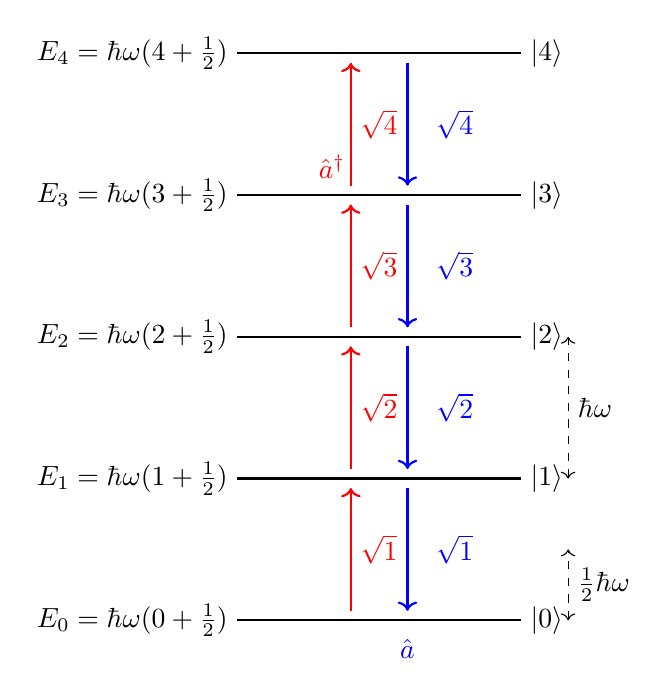
\begin{tikzpicture}[scale=1.2]
	% Niveles de energía
	\foreach \n in {0,1,2,3,4} {
		\draw[thick] (0,\n*1.5) -- (3,\n*1.5);
		\node[left] at (0,\n*1.5) {$E_{\n} = \hbar\omega(\n + \frac{1}{2})$};
		\node[right] at (3,\n*1.5) {$|{\n}\rangle$};
	}

	% Flechas de creación (rojas, hacia arriba)
\foreach \n in {0,1,2,3} {
	\pgfmathtruncatemacro{\m}{\n+1}
	\draw[->,red,thick] (1.2,\n*1.5+0.1) -- (1.2,\m*1.5-0.1);
	\node[red,right] at (1.2,\n*1.5+0.75) {$\sqrt{\m}$};
}
\node[red] at (1,4.8) {$\hat{a}^\dagger$};
		
		
		
		
		% Flechas de aniquilación (azules, hacia abajo)
	\foreach \n in {1,2,3,4} {
		\pgfmathtruncatemacro{\m}{\n-1}
		\draw[->,blue,thick] (1.8,\n*1.5-0.1) -- (1.8,\m*1.5+0.1);
		\node[blue,right] at (2,\n*1.5-0.75) {$\sqrt{\n}$};
	}
	\node[blue] at (1.8,-0.3) {$\hat{a}$};
	
	% Energía de punto cero
	\draw[<->,dashed] (3.5,0) -- (3.5,0.75);
	\node[right] at (3.5,0.375) {$\frac{1}{2}\hbar\omega$};
	\draw[<->,dashed] (3.5,1.5) -- (3.5,3);
	\node[right] at (3.5,2.25) {$\hbar\omega$};
	
\end{tikzpicture}

	\caption{Niveles de energía del oscilador armónico cuántico. Los operadores $\hat{a}^\dagger$ (rojo) y $\hat{a}$ (azul) actúan como escaleras, subiendo y bajando entre niveles con las constantes de normalización indicadas. El espaciado uniforme es $\hbar\omega$ y existe una energía de punto cero de $\frac{1}{2}\hbar\omega$. Fuente propia.}
	\label{fig:niveles}
\end{figure}




\subsection{Autofunciones del oscilador armónico en representación de posición}
\subsubsection{Autofunciones del oscilador armónico}

Los autoestados $|n\rangle$ obtenidos en la sección anterior son vectores abstractos en el espacio de Hilbert. Para calcular distribuciones de probabilidad y valores esperados de observables, necesitamos las \textbf{autofunciones} $\psi_n(x)$, que son las representaciones concretas de estos estados en el espacio de posición:

\begin{equation}
	\psi_n(x) = \langle x | n \rangle
\end{equation}

Las autofunciones son funciones de onda explícitas que podemos graficar y que satisfacen la ecuación de  \cite{schrodinger1926a} en forma de ecuación diferencial.

El resultado, derivado mediante el método analítico de \cite{schrodinger1926b} es:

\begin{equation}
	\psi_n(x) = \left(\frac{m\omega}{\pi\hbar}\right)^{1/4} \frac{1}{\sqrt{2^n n!}} H_n\left(\sqrt{\frac{m\omega}{\hbar}}x\right) \exp\left(-\frac{m\omega x^2}{2\hbar}\right)
	\label{eq:autofunciones}
\end{equation}

donde $H_n(\xi)$ son los polinomios de Hermite de orden $n$ (ver Apéndice~\ref{sec:hermite} para propiedades).


\subsubsection{Ortonormalidad}

Las autofunciones del oscilador armónico forman un conjunto \textbf{ortonormal}: son mutuamente ortogonales (perpendiculares en el sentido del producto interno) y cada una está normalizada (tiene norma unitaria). Matemáticamente:

\begin{equation}
	\int_{-\infty}^{\infty} \psi_n(x) \psi_m(x) dx = \delta_{nm}
\end{equation}

donde $\delta_{nm}$ es la delta de Kronecker:

\begin{equation}
	\delta_{nm} = \begin{cases} 
		1 & \text{si } n = m \\
		0 & \text{si } n \neq m
	\end{cases}
\end{equation}

\textbf{Ortogonalidad} ($n \neq m$): Funciones correspondientes a diferentes niveles de energía son mutuamente perpendiculares, reflejando que son estados físicamente distinguibles.

\textbf{Normalización} ($n = m$): Cada autofunción tiene probabilidad total igual a 1 de encontrar la partícula en algún lugar del espacio.


\subsubsection{Paridad}

Las funciones $\psi_n(x)$ tienen paridad bien definida:

\begin{equation}
	\psi_n(-x) = (-1)^n \psi_n(x)
\end{equation}

\textbf{Estados pares} ($n$ par): $\psi_n(-x) = +\psi_n(x)$ — función simétrica

\textbf{Estados impares} ($n$ impar): $\psi_n(-x) = -\psi_n(x)$ — función antisimétrica\\


\begin{figure}[h!]
	\centering
	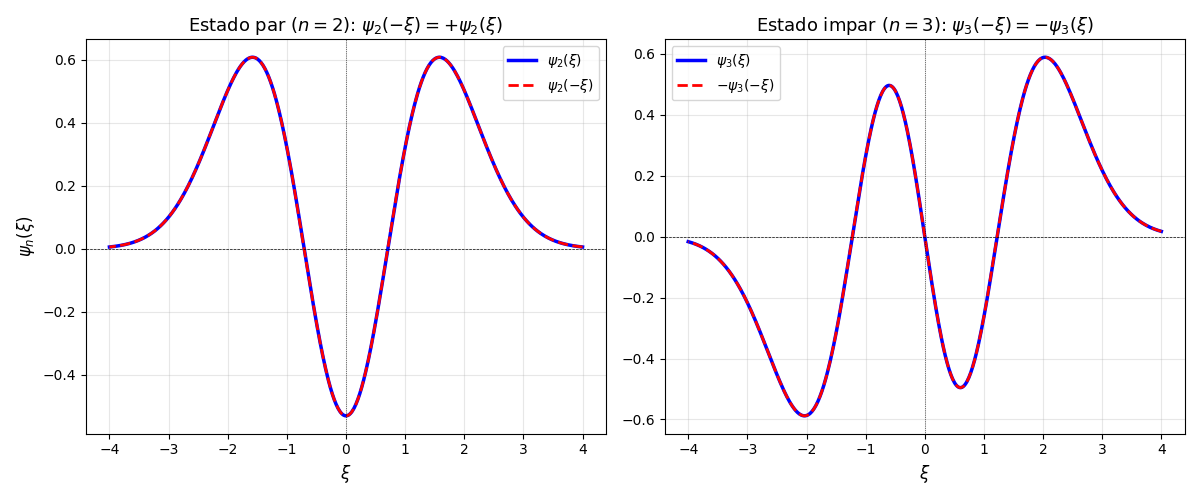
\includegraphics[width=1\linewidth]{paridad}
	\caption{Comparación paridad (estados pares vs impares). Fuente propia}
	\label{fig:paridad}
\end{figure}

\subsubsection{Número de nodos}

La función $\psi_n(x)$ tiene exactamente $n$ nodos (ceros):

\begin{itemize}
	\item $\psi_0(x)$: 0 nodos (gaussiana pura)
	\item $\psi_1(x)$: 1 nodo en $x = 0$
	\item $\psi_2(x)$: 2 nodos simétricos respecto al origen
	\item $\psi_n(x)$: $n$ nodos
\end{itemize}

Esta propiedad es general para problemas unidimensionales: el $n$-ésimo estado excitado tiene $n$ nodos.

\subsubsection{Funciones de onda de los primeros estados}

Usando la ecuación (\ref{eq:autofunciones}) y los primeros polinomios de Hermite (Apéndice ~\ref{sec:hermite}), obtenemos explícitamente:

\textbf{Estado fundamental ($n=0$):}
\begin{equation}
	\psi_0(x) = \left(\frac{m\omega}{\pi\hbar}\right)^{1/4} \exp\left(-\frac{m\omega x^2}{2\hbar}\right)
\end{equation}

Distribución gaussiana centrada en $x=0$ con ancho $\Delta x = \sqrt{\hbar/(2m\omega)}$.

\textbf{Primer estado excitado ($n=1$):}
\begin{equation}
	\psi_1(x) = \left(\frac{m\omega}{\pi\hbar}\right)^{1/4} \sqrt{\frac{2m\omega}{\hbar}} \, x \exp\left(-\frac{m\omega x^2}{2\hbar}\right)
\end{equation}

Función impar con un nodo en $x=0$.

\textbf{Segundo estado excitado ($n=2$):}
\begin{equation}
	\psi_2(x) = \left(\frac{m\omega}{\pi\hbar}\right)^{1/4} \frac{1}{\sqrt{2}}\left(\frac{2m\omega x^2}{\hbar} - 1\right) \exp\left(-\frac{m\omega x^2}{2\hbar}\right)
\end{equation}

Función par con dos nodos en $x = \pm\sqrt{\hbar/(2m\omega)}$.\\

\begin{table}[h]
	\centering
	\caption{Propiedades de los primeros estados del oscilador armónico cuántico}
	\label{tab:estados}
	\begin{tabular}{ccccl}
		\hline
		\textbf{Estado} & \textbf{Energía} & \textbf{Paridad} & \textbf{Nodos} & \textbf{Polinomio Hermite} \\
		$n$ & $E_n/(\hbar\omega)$ & Par/Impar & Cantidad & $H_n(\xi)$ \\
		\hline
		0 & 1/2 & Par & 0 & $1$ \\
		1 & 3/2 & Impar & 1 & $2\xi$ \\
		2 & 5/2 & Par & 2 & $4\xi^2 - 2$ \\
		3 & 7/2 & Impar & 3 & $8\xi^3 - 12\xi$ \\
		4 & 9/2 & Par & 4 & $16\xi^4 - 48\xi^2 + 12$ \\
		\hline
		\multicolumn{5}{l}{Patrón general: $E_n = \hbar\omega(n + \frac{1}{2})$, paridad = $(-1)^n$, nodos = $n$}
	\end{tabular}
\end{table}

	

\begin{figure}[H]
	\centering
	\includegraphics[width=0.8\linewidth]{"funciones de onda"}
	\caption{Ejemplos de funciones de onda $\psi_0, \psi_1, \psi_2, \psi_3$. Fuente propia}
	\label{fig:funciones-de-onda}
\end{figure}



\begin{figure}[H]
	\centering
	\includegraphics[width=0.8\linewidth]{"densidad de onda"}
	\caption{Ejemplos de densidades de probaiblidad $|\Psi_n|$ }
	\label{fig:densidad-de-onda}
\end{figure}



\subsection{Equivalencia entre el método analítico y el método algebraico}

Los métodos analítico y algebraico constituyen formulaciones matemáticamente equivalentes del mismo sistema físico. La identificación de esta equivalencia marcó uno de los hitos fundamentales en la consolidación de la mecánica cuántica, al demostrarse que la mecánica ondulatoria de Schrödinger y la mecánica matricial desarrollada por Heisenberg, Born y Jordan describen de manera consistente la misma estructura dinámica \citep{heisenberg1925, born1925, bornheisenberg1926, schrodinger1926a, schrodinger1926b}.


\subsubsection{Estado fundamental: comparación}

\textbf{Método analítico:} Para $n=0$, $H_0(\xi) = 1$, y la ecuación (\ref{eq:autofunciones}) da:

\begin{equation}
	\psi_0(x) = \left(\frac{m\omega}{\pi\hbar}\right)^{1/4} e^{-m\omega x^2/(2\hbar)}
\end{equation}

\textbf{Método algebraico:} La condición $\hat{a}|0\rangle = 0$ en representación de posición se traduce en:

\begin{equation}
	\sqrt{\frac{m\omega}{2\hbar}}\left(x + \frac{\hbar}{m\omega}\frac{d}{dx}\right)\psi_0(x) = 0
\end{equation}

Resolviendo esta ecuación diferencial ordinaria de primer orden:

\begin{equation}
	\frac{d\psi_0}{dx} = -\frac{m\omega}{\hbar} x \psi_0
\end{equation}

\begin{equation}
	\psi_0(x) = A e^{-m\omega x^2/(2\hbar)}
\end{equation}

Con normalización, $A = (m\omega/\pi\hbar)^{1/4}$.

\textbf{¡Ambos métodos dan la misma función!}

\subsubsection{Estados excitados: conexión}

En representación de posición, el operador $\hat{a}^\dagger$ actúa como \cite{dirac1930}:

\begin{equation}
	\hat{a}^\dagger \to \sqrt{\frac{m\omega}{2\hbar}}\left(x - \frac{\hbar}{m\omega}\frac{d}{dx}\right)
\end{equation}

Aplicando $(\hat{a}^\dagger)^n$ a $\psi_0(x)$ genera polinomios multiplicando la gaussiana, que son precisamente los polinomios de Hermite multiplicados por la constante apropiada \citep{sakurai2020}.

\subsubsection{Interpretación física}

\textbf{Método analítico \citep{schrodinger1926b}} :
\begin{itemize}
	\item Proporciona funciones de onda explícitas en representación de posición
	\item Visualización directa de densidades de probabilidad $|\psi_n(x)|^2$
	\item Útil para cálculos de valores esperados de observables
	\item Permite entender el comportamiento espacial de estados cuánticos
\end{itemize}

\textbf{Método algebraico \citep{dirac1930}} :
\begin{itemize}
	\item Más elegante y general
	\item No requiere resolver ecuaciones diferenciales
	\item Se generaliza fácilmente a otros sistemas
	\item Lenguaje natural para describir excitaciones (fonones, fotones) en sistemas de muchos cuerpos
	\item Lenguaje natural para describir excitaciones (fonones, fotones) en sistemas de muchos cuerpos y en teorías cuánticas de campos

\end{itemize}

\begin{table}[h]
	\centering
	\caption{Comparación entre el método analítico (Schrödinger) y algebraico (Dirac)}
	\label{tab:comparacion_metodos}
	\begin{tabular}{p{4cm}p{5cm}p{5cm}}
		\hline
		\textbf{Aspecto} & \textbf{Método analítico} & \textbf{Método algebraico} \\
		\hline
		Formulación & Ecuación diferencial & Álgebra de operadores \\
		Herramienta principal & Polinomios de Hermite & Operadores escalera $\hat{a}$, $\hat{a}^\dagger$ \\
		Resultado directo & Autofunciones $\psi_n(x)$ & Espectro $E_n$ y autoestados $|n\rangle$ \\
		Complejidad matemática & Alta (EDOs, series) & Media (álgebra) \\
		Visualización & Directa ($|\psi_n(x)|^2$) & Requiere proyección \\
		Generalización & Específica al OAC & Se generaliza fácilmente \\
		\hline
	\end{tabular}
\end{table}


A lo largo de esta sección hemos derivado completamente el espectro de energía $E_n = \hbar\omega(n + \frac{1}{2})$ y las autofunciones $\psi_n(x)$ del oscilador armónico cuántico mediante el método desarrollado por \cite{dirac1930} y entendimos las equivalencias con el método desarrollado por \cite{schrodinger1926b}. La equivalencia matemática de ambos enfoques confirma la consistencia interna de la mecánica cuántica y demuestra que diferentes formalismos pueden describir el mismo sistema físico. Esta dualidad ha sido fundamental en el desarrollo de la física cuántica moderna, desde la teoría cuántica de campos hasta las aplicaciones contemporáneas en computación cuántica.





\section{Aplicaciones físicas del oscilador armónico cuántico}
\subsection{Vibraciones atómicas y moleculares}

\subsection{Fonones y vibraciones colectivas en sólidos}

\subsection{Osciladores cuánticos como modos bosónicos fundamentales}
\chapter{Conclusiones}
En el presente trabajo se desarrolló el cálculo cuántico completo del oscilador armónico, obteniendo explícitamente su espectro energético y sus autofunciones, y analizando su significado físico dentro de la mecánica cuántica.\\

\textbf{Espectro de energía cuantizado:} Se derivó analíticamente el espectro discreto de energía $E_n = \hbar\omega(n + \frac{1}{2})$ mediante el formalismo algebraico de operadores escalera de \cite{dirac1930}. La cuantización surge naturalmente de las relaciones de conmutación $[\hat{a}, \hat{a}^\dagger] = 1$ y la condición de no negatividad del operador número $\langle n|\hat{N}|n\rangle = ||\hat{a}|n\rangle||^2 \geq 0$, estableciendo que los niveles energéticos están igualmente espaciados por $\hbar\omega$ y existe una energía de punto cero de $\frac{1   }{2}\hbar\omega$ incluso en el estado fundamental.\\
    
    
\textbf{Autofunciones y propiedades:} Se obtuvieron las autofunciones explícitas $\psi_n(x)$ expresadas en términos de polinomios de Hermite multiplicados por una envolvente gaussiana. Se caracterizaron sus propiedades fundamentales: ortonormalidad (asegurando que los estados son físicamente distinguibles), paridad bien definida según $(-1)^n$, y estructura nodal donde el $n$-ésimo estado presenta exactamente $n$ ceros, confirmando la relación entre nivel de excitación y complejidad espacial de la función de onda.\\

\textbf{Equivalencia de formalismos:} Se demostró la equivalencia matemática entre el método algebraico de \cite{dirac1930} y el método analítico de \cite{schrodinger1926a}, validando que ambos conducen a las mismas autofunciones para el estado fundamental y estados excitados. Esta equivalencia confirma la consistencia interna de la mecánica cuántica y evidencia que diferentes representaciones matemáticas describen la misma física subyacente. El método algebraico resulta más elegante y generalizable, mientras que el analítico proporciona visualización directa de las densidades de probabilidad.\\

\textbf{Importancia del oscilador armónico:} El sistema estudiado trasciende su valor como ejercicio académico. El formalismo de operadores de creación y aniquilación desarrollado constituye el lenguaje natural para describir excitaciones cuantizadas (fonones, fotones, plasmones) en sistemas de muchos cuerpos, y es fundamental en aplicaciones contemporáneas como circuit QED y códigos bosónicos para corrección de errores en computación cuántica. La solución del oscilador armónico cuántico representa así un puente conceptual entre los fundamentos teóricos establecidos por \cite{schrodinger1926a} y \cite{dirac1930} en la década de 1920 y las tecnologías cuánticas del siglo XXI.


%\cleardoublepage
\addcontentsline{toc}{chapter}{Bibliografía} 


%este esta ok
%\bibliographystyle{apalike} 
%\bibliography{referencias}



\bibliographystyle{apalike} % Estilo compatible con natbib y autor-año
\bibliography{referencias}   % Nombre de tu archivo .bib sin la extensión

\appendix
\chapter{Apéndices}

\section{Demostración de $[\hat{a}, \hat{a}^\dagger] = 1$} \label{sec:born1925}


Partimos de las definiciones:

\begin{align}
	\hat{a} &= \sqrt{\frac{m\omega}{2\hbar}}\left(\hat{x} + \frac{i}{m\omega}\hat{p}\right) \\
	\hat{a}^\dagger &= \sqrt{\frac{m\omega}{2\hbar}}\left(\hat{x} - \frac{i}{m\omega}\hat{p}\right)
\end{align}

Calculamos el conmutador $[\hat{a}, \hat{a}^\dagger] = \hat{a}\hat{a}^\dagger - \hat{a}^\dagger\hat{a}$:

\begin{align}
	\hat{a}\hat{a}^\dagger &= \frac{m\omega}{2\hbar}\left(\hat{x} + \frac{i}{m\omega}\hat{p}\right)\left(\hat{x} - \frac{i}{m\omega}\hat{p}\right) \\
	&= \frac{m\omega}{2\hbar}\left(\hat{x}^2 - \frac{i}{m\omega}\hat{x}\hat{p} + \frac{i}{m\omega}\hat{p}\hat{x} + \frac{1}{m^2\omega^2}\hat{p}^2\right) \\
	&= \frac{m\omega}{2\hbar}\hat{x}^2 + \frac{1}{2m\omega\hbar}\hat{p}^2 + \frac{i}{2\hbar}(\hat{p}\hat{x} - \hat{x}\hat{p})
\end{align}

El último término es $-\frac{i}{2\hbar}[\hat{x}, \hat{p}]$. Similarmente:

\begin{align}
	\hat{a}^\dagger\hat{a} &= \frac{m\omega}{2\hbar}\left(\hat{x} - \frac{i}{m\omega}\hat{p}\right)\left(\hat{x} + \frac{i}{m\omega}\hat{p}\right) \\
	&= \frac{m\omega}{2\hbar}\hat{x}^2 + \frac{1}{2m\omega\hbar}\hat{p}^2 + \frac{i}{2\hbar}[\hat{x}, \hat{p}]
\end{align}

Restando:

\begin{equation}
	[\hat{a}, \hat{a}^\dagger] = \hat{a}\hat{a}^\dagger - \hat{a}^\dagger\hat{a} = -\frac{i}{2\hbar}[\hat{x}, \hat{p}] - \frac{i}{2\hbar}[\hat{x}, \hat{p}] = -\frac{i}{\hbar}[\hat{x}, \hat{p}]
\end{equation}

Usando la relación de conmutación canónica de \cite{born1925}:

\begin{equation}
	[\hat{x}, \hat{p}] = i\hbar
\end{equation}

Obtenemos:

\begin{equation}
	[\hat{a}, \hat{a}^\dagger] = -\frac{i}{\hbar}(i\hbar) = -i^2 = 1
\end{equation}

\begin{equation}
	\boxed{[\hat{a}, \hat{a}^\dagger] = 1}
\end{equation}	
	
% APÉNDICE NUEVO: Factorización algebraica del hamiltoniano

 \section{Factorización algebraica del hamiltoniano}
 \label{sec:factorizacion}

 Sustituyendo las expresiones de $\hat{x}$ y $\hat{p}$ en términos de los
 operadores escalera:

\begin{equation}
 \hat{p}^2 = -\frac{m\omega\hbar}{2}(\hat{a}^\dagger - \hat{a})^2
           = -\frac{m\omega\hbar}{2}(\hat{a}^{\dagger 2} - \hat{a}^\dagger\hat{a}
             - \hat{a}\hat{a}^\dagger + \hat{a}^2)
\end{equation}

\begin{equation}
 \hat{x}^2 = \frac{\hbar}{2m\omega}(\hat{a} + \hat{a}^\dagger)^2
           = \frac{\hbar}{2m\omega}(\hat{a}^2 + \hat{a}\hat{a}^\dagger + \hat{a}^\dagger\hat{a} + \hat{a}^{\dagger 2})
\end{equation}

Sumando los términos $\frac{\hat{p}^2}{2m} + \frac{1}{2}m\omega^2\hat{x}^2$ y usando $[\hat{a},\hat{a}^\dagger]=1$, es decir,
$\hat{a}\hat{a}^\dagger = \hat{a}^\dagger\hat{a} + 1$:

\begin{equation}
\hat{H} = \hbar\omega\left(\hat{a}^\dagger\hat{a} + \frac{1}{2}\right)
         = \hbar\omega\left(\hat{N} + \frac{1}{2}\right)
\end{equation}

 Los términos cruzados $\hat{a}^2$ y $\hat{a}^{\dagger 2}$ se cancelan,
 y los términos $\hat{a}\hat{a}^\dagger + \hat{a}^\dagger\hat{a}
 = 2\hat{N} + 1$ producen el resultado final.


\section{Constantes de normalización: $\hat{a}^\dagger|n\rangle = \sqrt{n+1}|n+1\rangle$} \label{sec:normalizacion1}

Queremos determinar la constante de proporcionalidad cuando $\hat{a}^\dagger$ actúa sobre $|n\rangle$.

Sabemos que $\hat{a}^\dagger|n\rangle$ es proporcional a $|n+1\rangle$:

\begin{equation}
	\hat{a}^\dagger|n\rangle = c|n+1\rangle
\end{equation}

Para encontrar $c$, calculamos la norma al cuadrado:

\begin{equation}
	||\hat{a}^\dagger|n\rangle||^2 = \langle n|\hat{a}\hat{a}^\dagger|n\rangle
\end{equation}

Usando la relación de conmutación $\hat{a}\hat{a}^\dagger = \hat{a}^\dagger\hat{a} + 1$:

\begin{align}
	||\hat{a}^\dagger|n\rangle||^2 &= \langle n|(\hat{a}^\dagger\hat{a} + 1)|n\rangle \tag{A.14}\\
	&= \langle n|\hat{N}|n\rangle + \langle n|n\rangle \quad \text{(donde } \hat{N} = \hat{a}^\dagger\hat{a}\text{)} \tag{A.15}\\
	&= n + 1 \tag{A.16}
\end{align}

Por otro lado, si $\hat{a}^\dagger|n\rangle = c|n+1\rangle$:

\begin{equation}
	||\hat{a}^\dagger|n\rangle||^2 = |c|^2
\end{equation}

Igualando: $|c|^2 = n + 1$, entonces $c = \sqrt{n+1}$ (tomamos la raíz positiva por convención).

\textbf{Resultado:}

\begin{equation}
	\boxed{\hat{a}^\dagger|n\rangle = \sqrt{n+1}|n+1\rangle}
\end{equation}

	

\section{Constantes de normalización: $\hat{a}|n\rangle = \sqrt{n}|n-1\rangle$} \label{sec:normalizacion2}

De manera análoga, para $\hat{a}|n\rangle = d|n-1\rangle$:

\begin{align}
	||\hat{a}|n\rangle||^2 &= \langle n|\hat{a}^\dagger\hat{a}|n\rangle \\
	&= \langle n|\hat{N}|n\rangle \\
	&= n
\end{align}

Por lo tanto: $|d|^2 = n \implies d = \sqrt{n}$

\textbf{Resultado:}

\begin{equation}
	\boxed{\hat{a}|n\rangle = \sqrt{n}|n-1\rangle}
\end{equation}

\begin{table}[h]
	\centering
	\caption{Acción de los operadores escalera sobre autoestados}
	\label{tab:operadores_escalera}
	\begin{tabular}{ccc}
		\hline
		\textbf{Estado inicial} & \textbf{Operador creación} & \textbf{Operador aniquilación} \\
		& $\hat{a}^\dagger|n\rangle$ & $\hat{a}|n\rangle$ \\
		\hline
		$|0\rangle$ & $\sqrt{1}|1\rangle = |1\rangle$ & $0$ \\
		$|1\rangle$ & $\sqrt{2}|2\rangle$ & $\sqrt{1}|0\rangle = |0\rangle$ \\
		$|2\rangle$ & $\sqrt{3}|3\rangle$ & $\sqrt{2}|1\rangle$ \\
		$|3\rangle$ & $\sqrt{4}|4\rangle = 2|4\rangle$ & $\sqrt{3}|2\rangle$ \\
		$|n\rangle$ & $\sqrt{n+1}|n+1\rangle$ & $\sqrt{n}|n-1\rangle$ \\
		\hline
	\end{tabular}
\end{table}



\section{Polinomios de Hermite} \label{sec:hermite}

Los polinomios de Hermite $H_n(\xi)$ aparecen en las autofunciones del oscilador armónico cuántico. Este apéndice presenta sus propiedades esenciales.

\subsection{Definición}

Los polinomios de Hermite se definen mediante la fórmula de Rodrigues:

\begin{equation}
	H_n(\xi) = (-1)^n e^{\xi^2} \frac{d^n}{d\xi^n} e^{-\xi^2}
\end{equation}



\begin{figure}[h!]
	\centering
	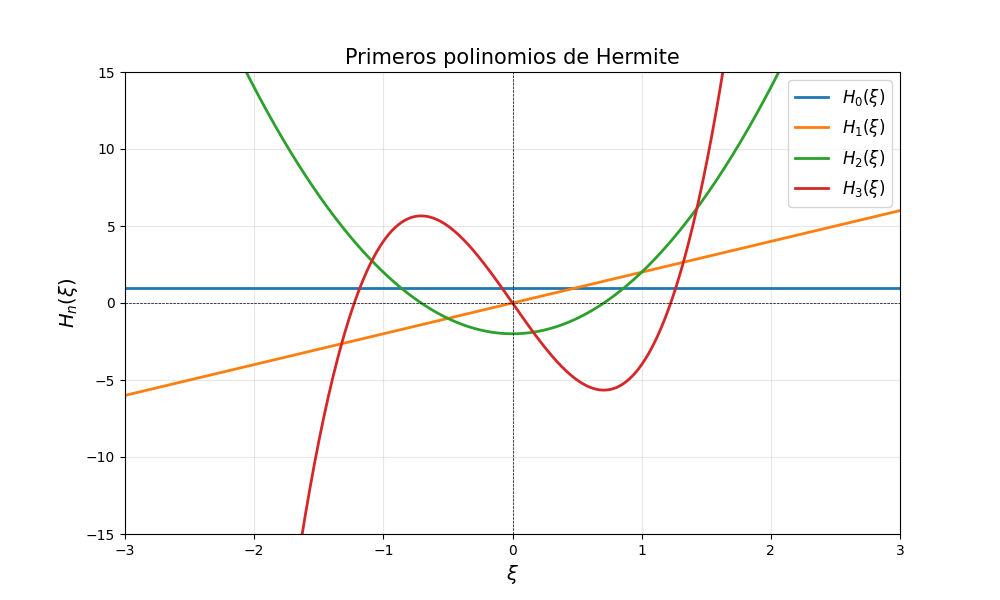
\includegraphics[width=0.9\linewidth]{hermite}
	\caption{Ejemplos de polinomios de Hermite $H_0, H_1, H_2, H_3$}
	\label{fig:hermite}
\end{figure}



\subsection{Primeros polinomios}

\begin{align}
	H_0(\xi) &= 1 \\
	H_1(\xi) &= 2\xi \\
	H_2(\xi) &= 4\xi^2 - 2 \\
	H_3(\xi) &= 8\xi^3 - 12\xi \\
	H_4(\xi) &= 16\xi^4 - 48\xi^2 + 12
\end{align}

\textbf{Propiedades generales:}
\begin{itemize}
	\item $H_n(\xi)$ es un polinomio de grado $n$
	\item El coeficiente del término de mayor grado es $2^n$
	\item Paridad: $H_n(-\xi) = (-1)^n H_n(\xi)$
\end{itemize}

\subsection{Relación de recurrencia}

Los polinomios se pueden generar mediante:

\begin{equation}
	H_{n+1}(\xi) = 2\xi H_n(\xi) - 2n H_{n-1}(\xi)
\end{equation}

Esta relación permite calcular $H_{n+1}$ conociendo $H_n$ y $H_{n-1}$.

\subsection{Ortogonalidad}

Los polinomios de Hermite son ortogonales con peso gaussiano:

\begin{equation}
	\int_{-\infty}^{\infty} H_n(\xi) H_m(\xi) e^{-\xi^2} d\xi = \begin{cases}
		0 & \text{si } n \neq m \\
		\sqrt{\pi} \, 2^n n! & \text{si } n = m
	\end{cases}
\end{equation}

Esta propiedad garantiza la ortonormalidad de las autofunciones del OAC cuando se incluye la constante de normalización apropiada:

\begin{equation}
	A_n = \left(\frac{m\omega}{\pi\hbar}\right)^{1/4} \frac{1}{\sqrt{2^n n!}}
\end{equation}

\subsection{Consecuencias para las autofunciones}

\textbf{Paridad:} Como $H_n(-\xi) = (-1)^n H_n(\xi)$, las autofunciones tienen paridad bien definida:
\begin{equation}
	\psi_n(-x) = (-1)^n \psi_n(x)
\end{equation}

Estados pares ($n$ par): funciones simétricas

Estados impares ($n$ impar): funciones antisimétricas

\textbf{Número de nodos:} El polinomio $H_n(\xi)$ tiene exactamente $n$ ceros reales. Por lo tanto, $\psi_n(x)$ tiene exactamente $n$ nodos.



\end{document}





















